\subsection{Data}
\subsubsection{Calibration Data}
\label{subsec:calibration-data}

Three sites in Switzerland (CH Bramenwies), western (Rur catchment, DE-Rur) and south-eastern Germany (Munich-North-Isar, DE-MNI) were used for calibration, i.e., for establishing the physiological a-priori knowledge. The data cover several winter wheat growing seasons. The sites represent winter wheat field parcels operated by farmers according to local agricultural management practice (see Table~\ref{tab:Calibration_data_overview} for an overview).

At all sites, \gls{GLAI} measurements (section \ref{subsubsec:glai-processing}) and phenology (section \ref{subsubsec:phenology-processing}) ratings were carried out, which were linked to hourly air temperature from nearby weather stations. The \gls{GLAI} measurements were chosen to represent the generative phase of the growing season, within which the \gls{GLAI} should increase over time, i.e., the beginning of stem elongation to heading. In total the calibration data set contains 890 data points with the corresponding temperature history (Table~\ref{tab:Calibration_data_overview}). The dataset contains a total of 11 environments (year $\times$ location), providing a representative data set for model calibration in temperate environments of central Europe. Further details about the sites are provided in the following paragraphs.

\begin{table}[H]
\caption{Calibration data with locations, years, the corresponding amount of \gls{GLAI} measurements, and reference of the dataset. Latitude and longitude are provided in geographic coordinates (WGS-84).}
\label{tab:Calibration_data_overview}

\centering
\begin{tabular}{llllll}
Location      & Years                                                                        & \begin{tabular}[c]{@{}l@{}}\gls{GLAI}\\measurements\end{tabular}  & Lat. & Lon. & Reference \\ \hline
CH Bramenwies & 2022  & 840   & 47.45 & 8.69     & ~\cite{wildhaber_assessing_2023}          \\
DE MNI        & \begin{tabular}[c]{@{}l@{}}2017, 2018,\\ 2020, 2021,\\ 2022\end{tabular} & 24   & 48.29 & 11.71 &  \begin{tabular}[c]{@{}l@{}}~\cite{danner_retrieval_2017},\\~\cite{danner_fitted_2019},\\~\cite{wocher_physically-based_2018}\end{tabular}         \\
DE Rur        & \begin{tabular}[c]{@{}l@{}}2008, 2009,\\ 2010, 2013,\\ 2015\end{tabular} & 26   &  50.87 & 6.44 & \cite{reichenau_comprehensive_2020}       \\
\hline
\end{tabular}
\end{table}

\paragraph{CH Bramenwies}
At the Bramenwies site in northern Switzerland ($47.45^\circ$ N, $8.69^\circ$ E, 550 m above sea level), 840 \gls{GLAI} were measured within a single winter wheat field parcel (2.04 ha) at 29 predefined sampling points during the growing season of 2022. The area receives a total annual precipitation of 1200 mm and has an annual air temperature of 10 °C (reference period 2011 to 2022). The soil of the moderately sloping parcel is loamy (clay content 20 to 30\%) and slightly alkaline (pH between 7.2 and 7.8) with moderate humus content (3.0 to 3.6\%). The parcel was managed according to Swiss standards for conventional agriculture with three applications of mineral fertiliser in April and May 2022 \citep{wildhaber_assessing_2023}. Meteorological data were available from a weather station operated by the Agrometeorological Network of the Institute for Excellence in Agricultural Research, Agroscope.

\paragraph{DE MNI}
24 \gls{GLAI} measurements in winter wheat from five years between 2017 and 2022 were available at the MNI site ($48.29^\circ$ N, $11.71^\circ$ E, 440 m above sea level) close to the river Isar ($\le$ 10 km) north of the city of Munich. Measurements were taken between the beginning of April and July each year. The average annual air temperature is about 8.9 degrees Celsius with an annual precipitation of 757 mm (reference period 1991 to 2020). The dominant soil types in the mostly flat area are gleysols and pararendzina of alluvial origin. The parcels were managed according to conventional agricultural practices following German standards \citep{danner_retrieval_2017, danner_fitted_2019, wocher_physically-based_2018}. Weather data was obtained from a station operated by the German Meteorological Service at Munich Airport.

\paragraph{DE Rur}
At the Rur catchment in northwestern Germany, 26 \gls{GLAI} measurements were made in five years between 2008 and 2015 ($50.87^\circ$ N, $6.44^\circ$ E, 100 m above sea level) in a fertile loess plain characterised by luvisols and anthrosols \citep{reichenau_comprehensive_2020}. From the original dataset of \cite{reichenau_comprehensive_2020} we took \gls{GLAI} observations in winter wheat from the sites Merzenhausen, Selhausen and Merken. The mean annual air temperature at these sites is about 10 degrees C and the total annual precipitation is about 700 mm. The fields were managed conventionally according to local best agricultural practice. Weather data were measured at stations located close to the monitored plots.

\subsection{Validation Data}
\label{subsec:validation-data}
Independent data to validate the reconstructed \gls{GLAI} time series were collected in 2022 and 2023 on seven winter wheat parcels at the Strickhof and Swiss Future Farm sites in northern Switzerland. The location of the sites and the shapes of the field plots are shown in Figure ~\ref{fig:map-validation-sites}a.  A sampling design of between three and eight sampling points per parcel was chosen to capture the heterogeneity within fields (white dots in Figure~\ref{fig:map-validation-sites}a). All sites are located in the Swiss Central Plateau, which is characterised by a temperate climate (mean annual air temperature around 10°C) and humid conditions (annual precipitation around 1000 mm). Both sites are equipped with weather stations operated by the Swiss Federal Office of Meteorology and Climatology, MeteoSwiss (Swiss Future Farm) and the AgroMeteo network of the Swiss Federal Centre of Excellence for Agricultural Research, Agroscope (Strickhof), which provide hourly air temperature measurements.

The fields were managed according to Swiss conventional agricultural practice. Detailed management information including the sowing date, winter wheat variety as well as timing and amount of fertilizer applied was provided by the farmers.

\begin{figure}[H]
    \centering
    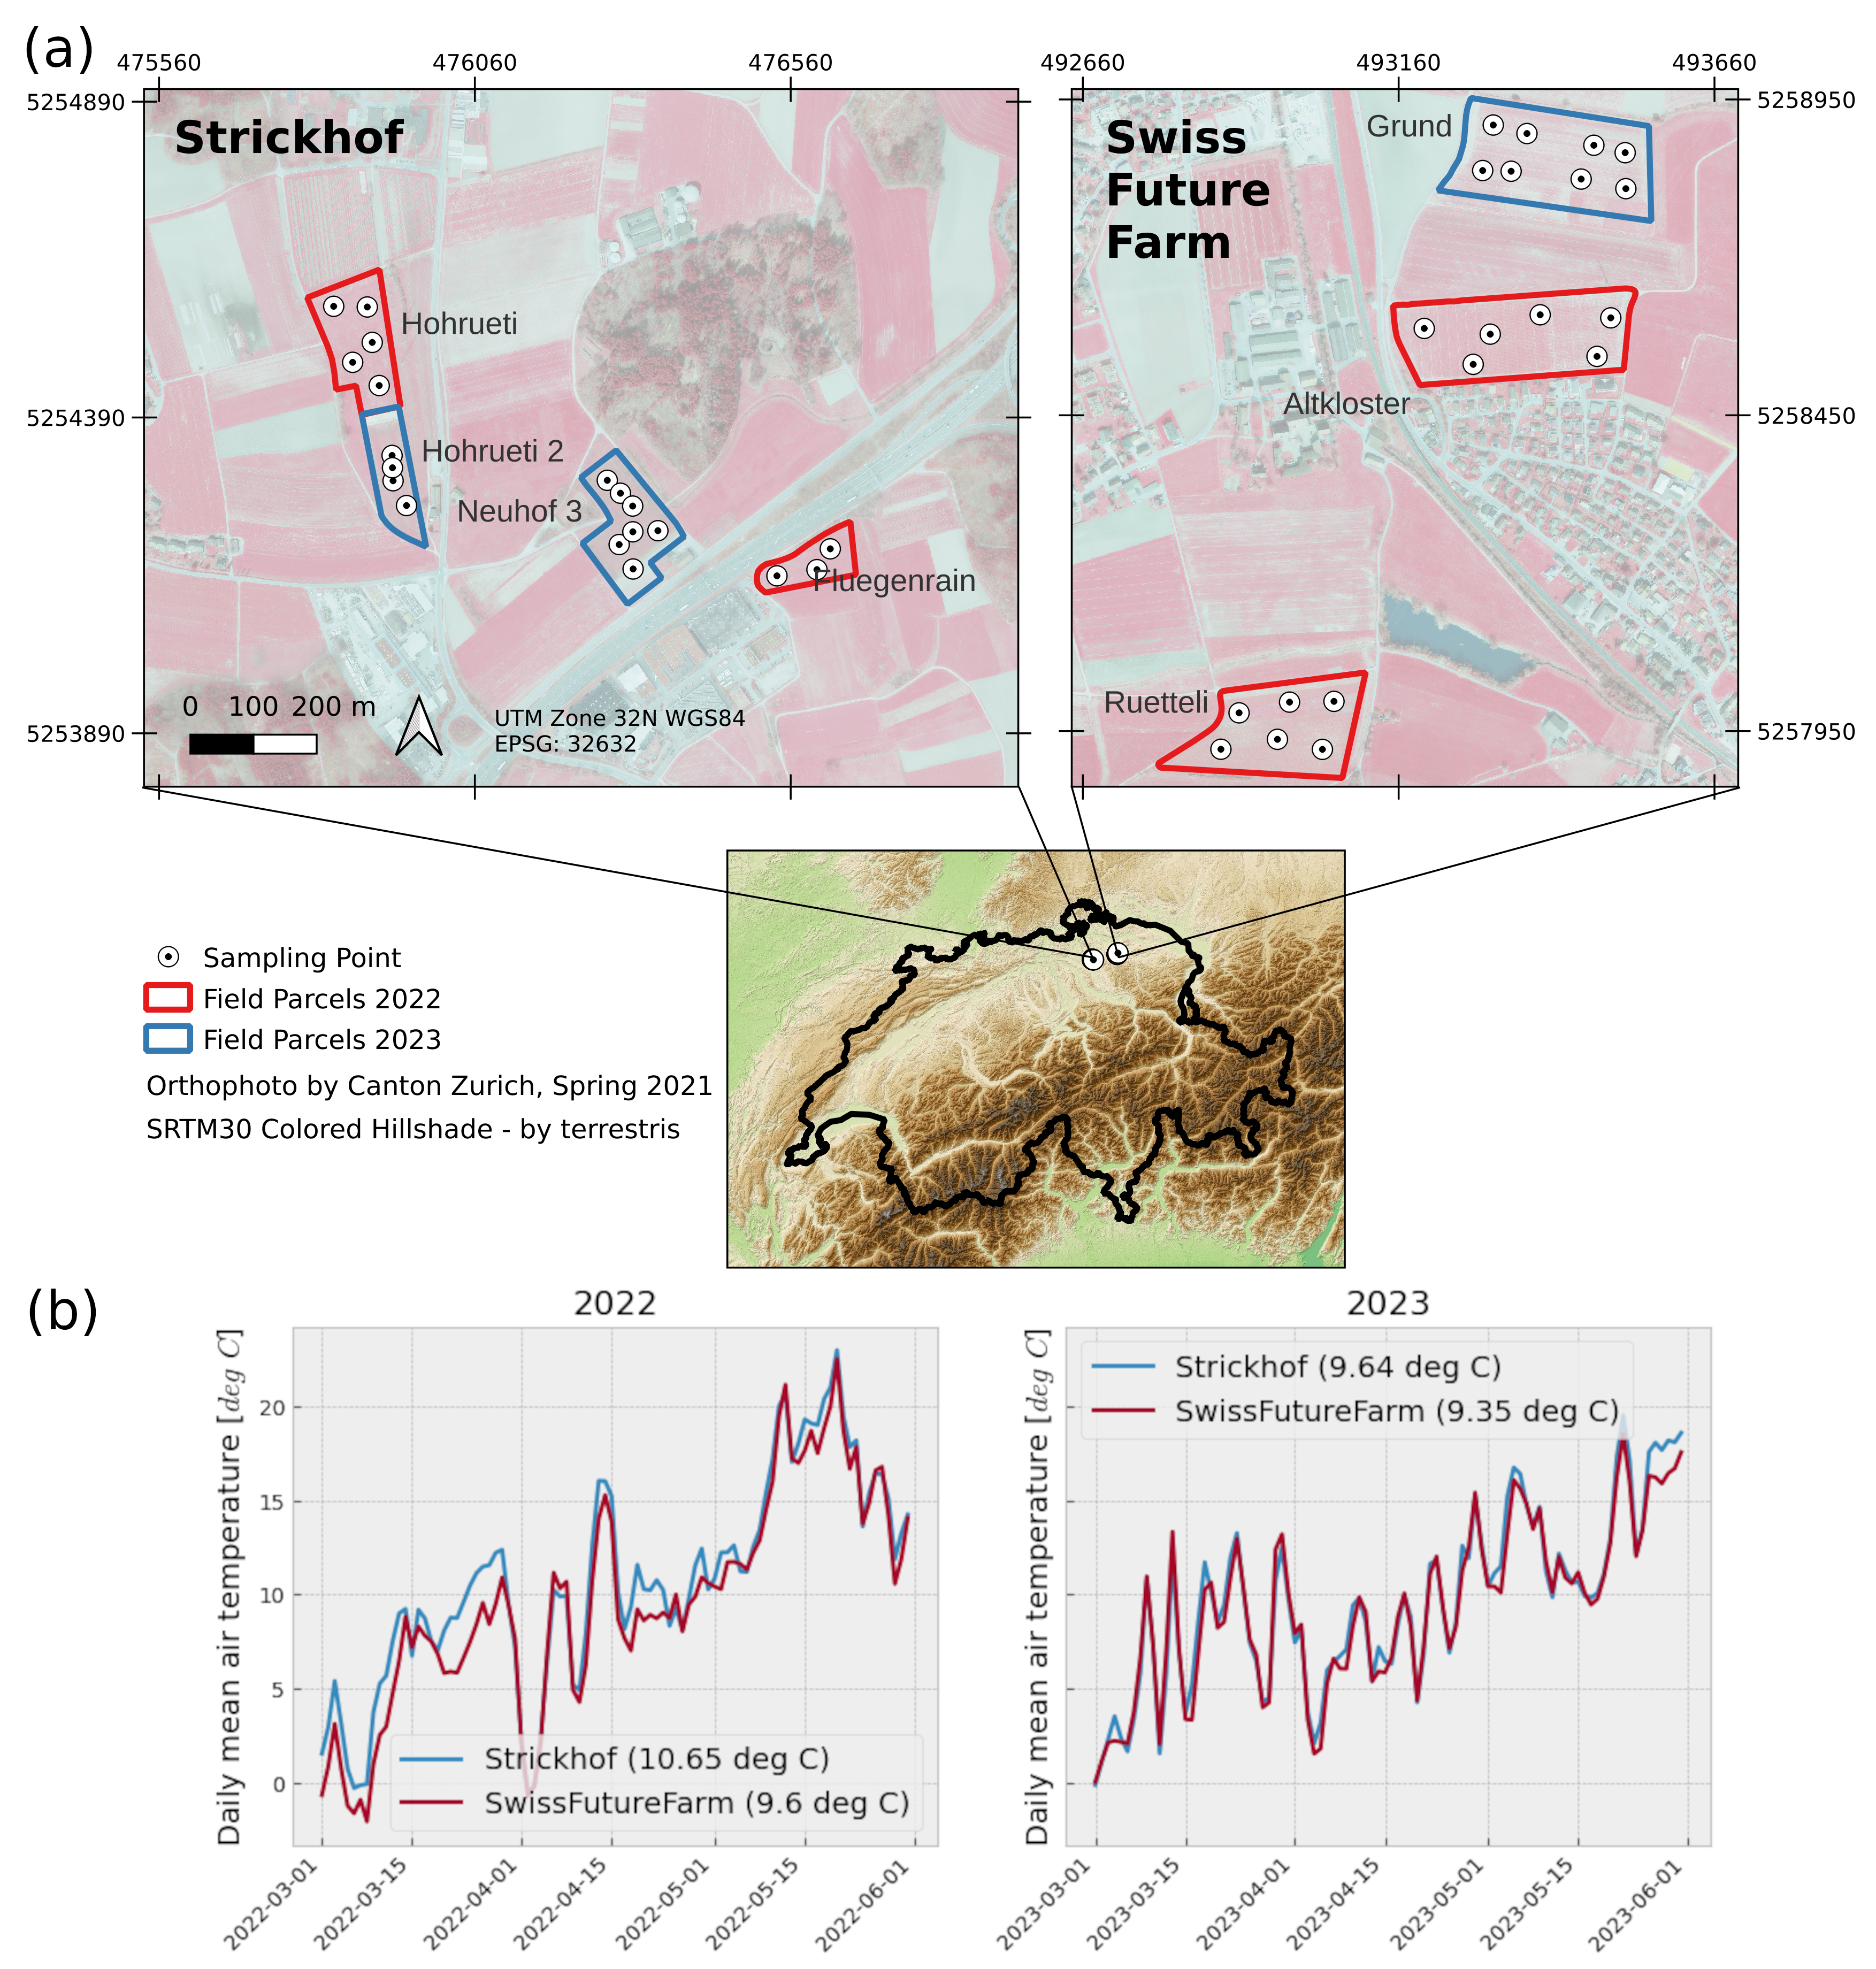
\includegraphics[width=1.0\textwidth]{overview_validation_sites_and_meteo.png}
    \caption{(a) Map of the two sites at which independent validation data was acquired in 2022 (red) and 2023 (blue). Dots denote the position of the sampling points in the field parcels to capture field heterogeneity. (b) Daily mean air temperature 2 m above ground at the validation sites in spring 2022 (left) and 2023 (right). The mean air temperature between 1st of March and 30th of June is given in the legend in brackets.}
    \label{fig:map-validation-sites}
\end{figure}

In terms of meteorology, 2022 and 2023 were different: 2022 had a dry and warm spring, while April and May of 2023 were rainy and higher temperatures only occurred towards the end of May. Figure~\ref{fig:map-validation-sites}b shows the daily mean air temperatures for the Strickhof (blue) and Swiss Future Farm (red) sites in 2022 (left) and 2023 (right). In both years the Strickhof site was warmer than the Swiss Future Farm site. In 2022, the mean air temperature between the beginning of March and June was 10.65 and 9.6 degrees C for Strickhof and Swiss Future Farm, respectively. In 2023 this value decreased to 9.64 and 9.35 degrees C respectively.

\subsection{Sentinel-2 Imagery}
\label{subsec:s2-imagery}
Thanks to its twin-constellation of \gls{S2}A and B, the \gls{S2} platform provides high revisit rates (<= 5 days in mid-latitudes) and captures spectral reflectance data in 13 channels between 490 and 2200 nm in up to 10 m spatial resolution. \gls{S2} has therefore proven an invaluable data source for vegetation studies including the retrieval of crop functional traits~\citep[for instance]{amin_prototyping_2021,delloye_retrieval_2018}.

We obtained \gls{S2} bottom-of-atmosphere (processing level: L2A) imagery from Microsoft Planetary Computer\footnote{\url{https://planetarycomputer.microsoft.com/}} using the open-source Python library EOdal~\citep{graf_eodal_2022} (version 0.2.1; Python 3.10). The data cover the validation sites (Figure~\ref{fig:map-validation-sites}). We used all scenes in 2022 and 2023 between the beginning and ending of the stem elongation phase (i.e., April to June) with a scene-wide cloud cover threshold of $\le$ 50\%. We determined the date range considered per parcel from the in-situ ratings of phenology (Section~\ref{subsubsec:phenology-processing}). In addition, we used a scene before and after the determined time period to provide enhanced temporal context and account for uncertainty regarding the exact onset of the phenological development stages. In total, 17 \gls{S2} scenes were available at the Strickhof site in 2022 and 14 in 2023, while at the Swiss Future Farm site 14 and 11 scenes could be used in 2022 and 2023, respectively.
